\documentclass[12pt]{article} % The document class with options

\usepackage[margin=1in]{geometry}
\usepackage[utf8]{inputenc} 
\geometry{a4paper}
\usepackage{newtxtext,newtxmath}
\usepackage[T1]{fontenc}
\usepackage{amsmath}
\usepackage{amsfonts}
\usepackage{microtype}
\usepackage{graphicx}
\usepackage{listings} % For formatting and highlighting code
\usepackage{color}    % For colors in code highlighting
\usepackage{hyperref}

% Define colors for syntax highlighting
\usepackage{color}
\definecolor{dkgreen}{rgb}{0,0.6,0}
\definecolor{gray}{rgb}{0.5,0.5,0.5}
\definecolor{mauve}{rgb}{0.58,0,0.82}

% Code listing style named "mystyle"
\lstset{frame=tb,
  language=Python,
  aboveskip=3mm,
  belowskip=3mm,
  showstringspaces=false,
  columns=flexible,
  basicstyle={\small\ttfamily},
  numbers=none,
  numberstyle=\tiny\color{gray},
  keywordstyle=\color{blue},
  commentstyle=\color{dkgreen},
  stringstyle=\color{mauve},
  breaklines=true,
  breakatwhitespace=true,
  tabsize=3
}
% chktex-file 3
% chktex-file 8
% chktex-file 10
% chktex-file 17
% chktex-file 18
% chktex-file 36
% chktex-file 44

\begin{document}
\setlength{\parskip}{1em} 
\setlength{\parindent}{0pt}
\newcommand{\vect}[1]{\mathbf{#1}}
\section*{Question 4}
\subsection*{Part 1}
\begin{align*}
    \sigma_{\theta\theta}(r=a) &= 0\\
    \sigma_{r\theta}(r=a) &= 0\\
\end{align*}
\subsection*{Part 2}
\begin{align*}
    \sigma_{rr}(\frac{r}{a}=\infty ) &= \sigma_{0} \sin^{2}{\left(\theta \right)}\\
    \sigma_{r\theta}(\frac{r}{a}=\infty ) &= - \frac{\sigma_{0} \sin{\left(2 \theta \right)}}{2}\\
    \sigma_{\theta\theta}(\frac{r}{a}=\infty ) &= \sigma_{0} \sin^{2}{\left(\theta \right)}\\
\end{align*}
\subsection*{Part 3}
\begin{align*}
    \sigma_{xx}(\frac{r}{a}=\infty ) &= - \sigma_{0} \sin^{2}{\left(\theta \right)} \cos{\left(2 \theta \right)}\\
    \sigma_{yy}(\frac{r}{a}=\infty ) &= - \frac{\sigma_{0} \sin{\left(4 \theta \right)}}{4}\\
    \sigma_{xy}(\frac{r}{a}=\infty ) &= - \sigma_{0} \sin^{2}{\left(\theta \right)} \cos{\left(2 \theta \right)}\\
\end{align*}
\newpage
\subsection*{Part 4}
\begin{figure}[ht]
    \centering
    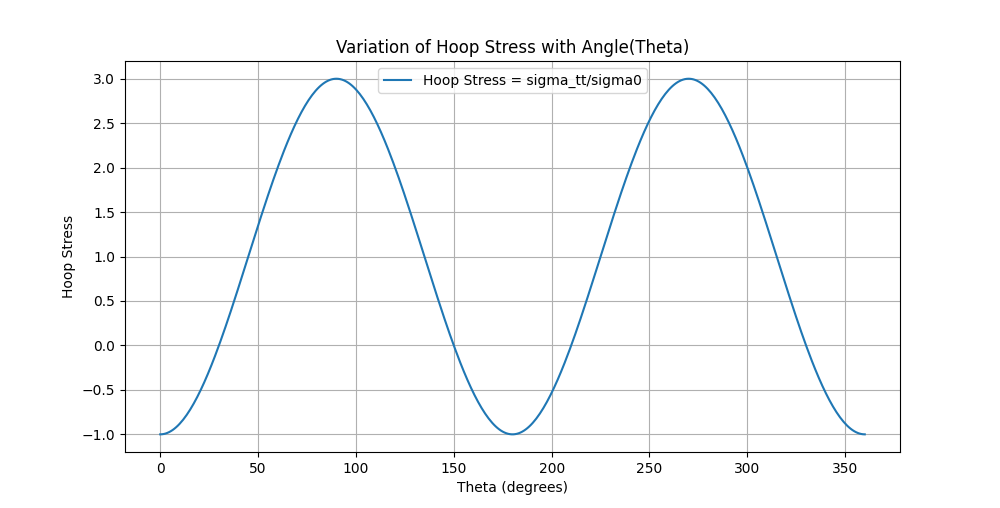
\includegraphics[width=1\textwidth]{Hoop Stress.png}
    \caption{Hoop Stress vs. Angle($\theta$)}
\end{figure}
The maximum value of hs is 3, which occurs at $\theta$ = 90.0 degrees.
\subsection*{Python Code for Q4}
\begin{lstlisting}
from sympy import symbols,log, diff,cos,sin,simplify,oo,limit,solveset,pi,Interval,latex
import matplotlib.pyplot as plt
import numpy as np


sigma0, a, r, theta = symbols('sigma0 a r theta')

phi = -0.5*sigma0*a**2*log(r) + 0.25*sigma0*r**2 + 0.25*sigma0*(2*a**2 - r**2 - a**4/(r**2))*cos(2*theta)

dphi_dr = diff(phi,r)
dphi_dtheta = diff(phi,theta)
d2phi_dr2 = diff(dphi_dr,r)
d2phi_dtheta2 =diff(dphi_dtheta,r)
d2phi_drt = diff(dphi_dr,theta)
LHS = (d2phi_dr2 + 1/r*dphi_dr + 1/(r**2)*d2phi_dtheta2)**2

sigma_rr = 1/r*dphi_dr + 1/(r**2)*d2phi_dtheta2
sigma_rtheta = (1/r**2)*dphi_dtheta-1/r*d2phi_drt #- diff((1/r)*dphi_dtheta,r)
sigma_tt = d2phi_dr2

# Part 1 r = a
s_rr_eva = sigma_rr.subs({r:a})
s_rt_eva = sigma_rtheta.subs({r:a})
print('Part 1')
print('sigma_rr (r=a) =', latex(simplify(s_rr_eva)))
print('sigma_rt (r=a) =', latex(simplify(s_rt_eva)))

# Part 2 r/a-->inf
s_rr_eva2 = limit(sigma_rr,r,oo)
s_rt_eva2 = limit(sigma_rtheta,r,oo)
s_tt_eva2 = limit(sigma_tt,r,oo)
print('Part 2')
print('sigma_rr (r/a=inf) =', latex(simplify(s_rr_eva2)))
print('sigma_rt (r/a=inf) =', latex(simplify(s_rt_eva2)))
print('sigma_tt (r/a=inf) =', latex(simplify(s_tt_eva2)))

# Part 3 x&y-->inf
# for the convertion from sigma_rr to sigma_xx, see the reference
sigma_xx = (sigma_rr * sin(theta) + sigma_rtheta * cos(theta))*sin(theta) + (sigma_rtheta * sin(theta) + sigma_tt * cos(theta))*cos(theta)
sigma_yy = (sigma_rr * cos(theta) + sigma_rtheta * sin(theta))*sin(theta) + (sigma_rtheta * cos(theta) + sigma_tt * sin(theta))*cos(theta)
sigma_xy = (sigma_rr * sin(theta) + sigma_rtheta * cos(theta))*sin(theta) + (sigma_rtheta * sin(theta) + sigma_tt * cos(theta))*cos(theta)
s_xx_eva = limit(sigma_xx,r,oo)
s_yy_eva = limit(sigma_yy,r,oo)
s_xy_eva = limit(sigma_xy,r,oo)
print('Part 3')
print('sigma_xx (x&y=inf) =', latex(simplify(s_xx_eva)))
print('sigma_yy (x&y=inf) =', latex(simplify(s_yy_eva)))
print('sigma_xy (x&y=inf) =', latex(simplify(s_xy_eva)))
print('Part 4')
import sympy as sp

# Part 4 
print('Part 4')
hs = sigma_tt / sigma0
hs_eva = hs.subs(r, a)
theta_radians = np.radians(np.linspace(0, 360, 400))
hs_values = [hs_eva.subs(theta, rad).evalf() for rad in theta_radians]

# Differentiating and solving for critical points
hs_prime = sp.diff(hs_eva, theta)
critical_points = sp.solveset(hs_prime, theta, domain=sp.Interval(0, 2 * sp.pi))

# Checking and evaluating at critical points
max_value = -float('inf')
theta_max = 0
if isinstance(critical_points, sp.FiniteSet):
    for point in critical_points:
        # Ensure that point is real
        if point.is_real:
            value = hs_eva.subs(theta, point).evalf()
            if value > max_value:
                max_value = value
                theta_max = point

# Convert theta_max from radians to degrees
if theta_max != 0:  # Check to ensure theta_max was set
    theta_max_degrees = np.degrees(float(theta_max))
    print(f"The maximum value of hs is {max_value}, which occurs at theta = {theta_max_degrees} degrees.")
else:
    print("No real critical points found within the domain.")



plt.figure(figsize=(10, 5))
plt.plot(np.linspace(0, 360, 400), hs_values, label=f'Hoop Stress = sigma_tt/sigma0')
plt.title('Variation of Hoop Stress with Angle(Theta)')
plt.xlabel('Theta (degrees)')
plt.ylabel('Hoop Stress')
plt.grid(True)
plt.legend()
plt.show()
\end{lstlisting}
\subsection*{Reference for Q4}
\href{https://www.brown.edu/Departments/Engineering/Courses/En221/Notes/Polar_Coords/Polar_Coords.htm}{Reference Link}


\section*{Question 5}
\begin{align*}
    r_2 &= 0.05 \\
    r_1 &= 0.025 \\
    p_1 &= 0 \text{forccase 2} = 5e6 \text{forccase 1} \\
    p_2 &= -5e6 \text{forccase 2} = 0 \text{forccase 1} \\
\end{align*}
\begin{figure}[ht]
    \centering
    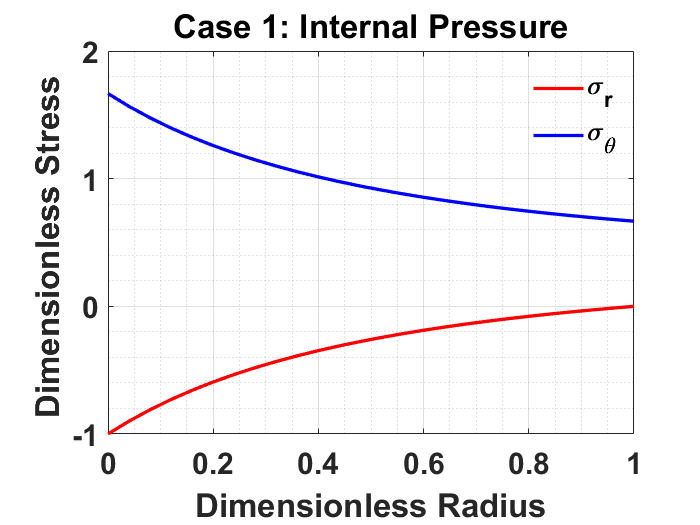
\includegraphics[width=1\textwidth]{case1.png}
    \caption{Case 1}
\end{figure}
\begin{figure}[ht]
    \centering
    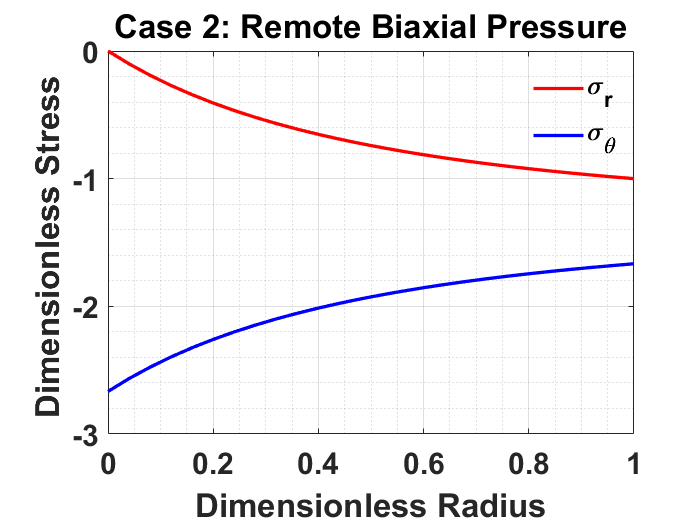
\includegraphics[width=1\textwidth]{case2.png}
    \caption{Case 2}
\end{figure}

Lastly, though in the statement of all the problems, validation with FEM solvers are required, I actually do not have access to Abaqus or Ansys at this moment, so the validation part remains for future work.
\end{document}